\chapter{Architectural proposal}
\label{chap:archimpl}
 
In this chapter we dig into the actual architectural proposal, seeing all the
problems related to it and how they were solved. We will show all the various
attempts made, and we will discussion about the technological issues and changes
we had to perform.

\section{Architecture introduction}

Before digging into the details of the actual implementation, we briefly
introduce some of its functional components and the way they work.

\subsection{A two-level orchestration framework}
\begin{figure}[t]
  \centering
  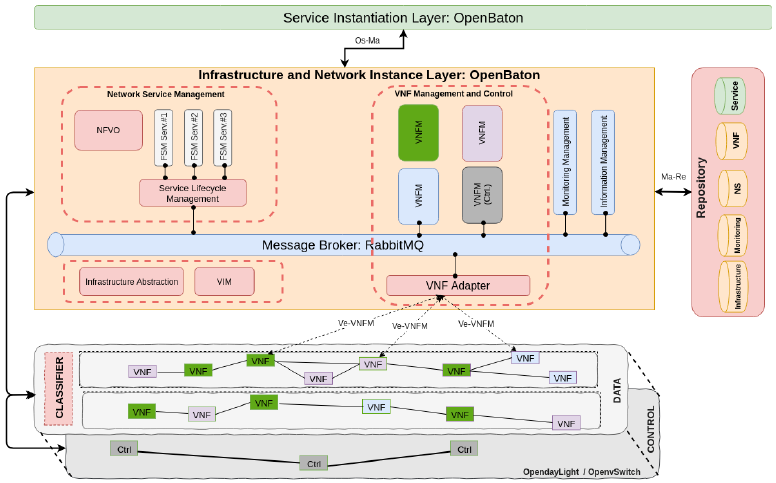
\includegraphics[width=\textwidth]{Architecture}
  \caption[Architecture schema depicting the expected
    implementation]{Architecture schema depicting the expected implementation.
    It is possible to see how Openbaton interacts with the various components in
    the architecture, and how RabbitMQ is used as a message broker between the
    different parts to enable message exchanging.}
  \label{chap:archimpl:sec:fistattempt:img:architecture}
\end{figure}

It is important to keep in consideration that the ETSI NFV architectural
framework is to be considered service and/or application agnostic. This excludes
this framework from the burden of being application aware for any possible NS
configuration and management, and for the VNF application layer configuration
and management.

The lack of these two management requires a service aware software, that has the
task to perform service lifecycle management and monitoring via the API offered
by the ETSI MANO. In this context, is possible to identify two different types
of orchestrators, as represented in
Figure~\ref{chap:archimpl:sec:fistattempt:img:architecture}:
\begin{itemize}
\item a high layer, service-aware;
\item a low layer, service-unaware.
\end{itemize}
Both layers rely on the Openbaton NFVO. The messages would be exchanged through
RabbitMQ, using the Advance Message Queuing Protocol (AMQP).

\paragraph*{Low-layer orchestrator}
The low-layer orchestrator job corresponds to the one defined in the ETSI MANO
definition, with the role of managing and orchestrating VNFs and NSs. The
low-layer MANO holds different data repositories where VNF and NS definitions
are stored, alongside with various monitoring tools, logs and network services
repositories. The low layer MANO exposes a set of APIs to the upper layer
(related to handling services) MANO, that is able to configure and manage the
services. In other words, the service MANO has the possibility to configure and
launch services to the low-layer orchestrator, providing the necessary
information.

\subsection{Low-layer functional components}
In the following section we are going to briefly talk about the role of the most
peculiar components in the defined architecture. A detailed description of the
tasks that the components have to abide in the ETSI MANO architecture is
available in Section~\ref{chap:archimpl:sec:secondattempt:sec:k8s}.
\begin{description}
\item[VNFM] As is possible to see from the
  Figure~\ref{chap:archimpl:sec:fistattempt:img:architecture}, the following
  architecture envisages the possibility of multiple VNFM components, required
  for the control and management of different virtualized functions. In
  particular, the use of different and specialized VNFMs allows to control and
  manage different functional aspects of the control/data plan.
\item[Network service management] in this architectural proposal, the Network
  service management corresponds to the brain of the infrastructure MANO, where
  service instantiation and lifecycle management happens. This part interacts
  with the VNFM/VIM and with the RabbitMQ middleware. In this context, the NFVO
  is involved in chaining the required VNFs in order to create the service
  delivery path. Inside this component is possible to identify the Service
  Lifecycle Management, that listens to status report coming from the VNFM and
  it generates logs and monitoring information.
\item[Monitoring and Information Management] this block gathers data from the
  data layers (identified in the image as the repository), which can be object
  of consultation from other applications.
\end{description}

From now on we are going to describe out attempt in implementing the
aforementioned architectural proposal, and we will describe the challenges and
the issue we encountered.

\section{First attempt}

In our first attempt we started building our infrastructure on top of Ubuntu
16.04 (for Openstack) and Ubuntu 18.04 (for Openbaton). Our main goal was to set
up Openstack as our VIM while setting Openbaton as our MANO. Then, Openbaton
would have registered Openstack as PoP, where TOSCA definitions would have been
launched on Openstack that, instead of deploying hypervisor based virtual
machines, it would have deployed container instances. The VNFs lifecycles would
have been controlled through an Element Management System (EMS), transmitting
the various VNF states via the message broker RabbitMQ. It is possible to see the
interactions between elements in a minimum schema available in
Figure~\ref{chap:archimpl:sec:fistattempt:img:schema1}.

\begin{figure}[t]
  \centering
  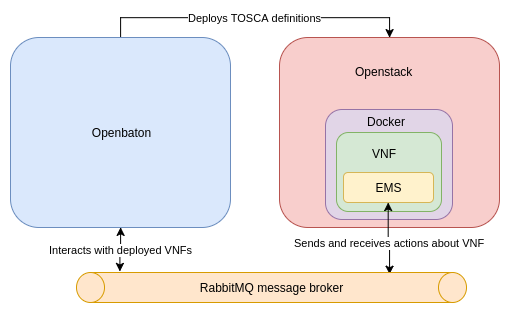
\includegraphics[scale=0.5]{Attempt1}
  \caption[Fist attempt components organization schema]{Fist attempt components
    organization schema. We can see how the main Openstack role is to deploy and
    manage the resources, while Openbaton has the role of management and
    orchestration. Finally, RabbitMQ sends and receives status update from the
    EMS for every VNF deployed.}
  \label{chap:archimpl:sec:fistattempt:img:schema1}
\end{figure}

\subsection{Openstack for container orchestration}

Our first step was to try and use Openstack to create a container orchestration.
The reason behind this approach was simple: Openbaton, on the paper, comes with
an out-of-the-box support for Openstack. In fact, it natively supports Openstack
PoPs, giving to us a great possibility to reuse the two frameworks and to ease
the development phase of our software.
\subsubsection{Devstack: Openstack for developers}
Openstack is composed by modules, giving the possibility to the user who wants
to install it to choose only the components it really needs. So the first thing
we decided was to perform a selection of these modules between the 33 available
in the installation page. The installation of this components span between
multiple machines (nodes), therefore creating a whole cluster of resources.
Since we considered too time-consuming to install Openstack in a distributed
manner, we considered to test first the developer version, called
\emph{Devstack}. Devstack offers the possibility to install a subset of modules
in the local machine, and to leverage a Openstack environment able to perform
the same operations of the production-grade installation. Thus, we started
configuring the Devstack installation, installing first of all the Nova module,
that is required to perform computing operations such as the launch of virtual
machines, and lately we installed Tacker too.

\paragraph*{Tacker}
\begin{figure}[t]
  \centering
  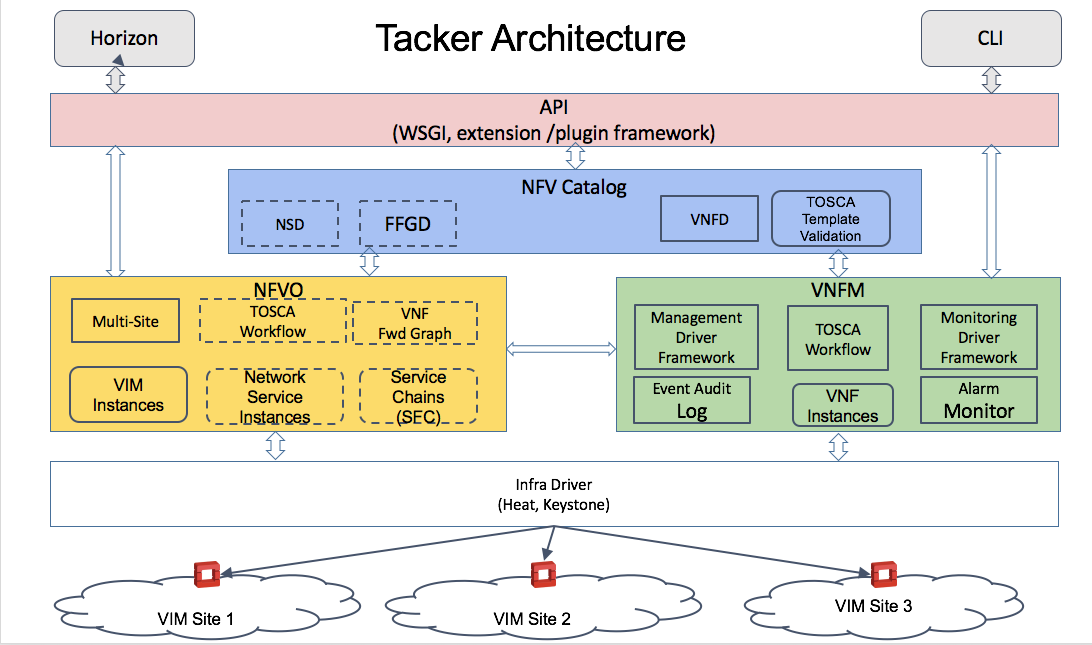
\includegraphics[scale=0.3]{tacker_architecture}
  \caption[Taker architecture schema]{Taker architecture
    schema~\cite{tackerOpenstackwiki}}
\end{figure}
Tacker is a VNFM and a NFVO. It is an official Openstack module, and it has the
ability to deploy, edit, stop and do periodic VNF health checks directly on it.
The developers claim it has the possibility to make deployments to platforms
compatible with Openstack too. It supports VNF definition through the TOSCA
standard, and a proposal for SFC integration has been made in
2015~\cite{tackerOpenstackwiki}.

We tried Tacker to see if its functionalities were good enough to be adopted in
our testbed instead of Openbaton. Its complete integration with Openstack,
indeed, was the main reason for its testing. At the end though, we felt like the
product was not ready for a real production environment. SFC management and the
lack of support for alternative platforms other than Openstack was another
reason to prefer Openbaton eventually.

\paragraph*{Devstack configuration}
The Openstack installation is not an easy one, particularly for newcomers, that 
have to deal with a great set of tools and not-always-clear instructions. Here 
we will describe how we managed to get a single-node deployment up and running.

First of all, Devstack needs a machine with at least 16GB of ram and 50GB of HD 
space.
We decided to install these components:
\begin{itemize}
 \item Keystone (for identity management)
 \item Object storage
 \item Compute
 \item Tacker (we tested this module to see is Openstack was a suitable VIM too)
\end{itemize}

Using Devstack is a simple operation, but the time required to reach a correct 
configuration is very high. In particular, it required from 20 minutes to 1 
hour to install Devstack with a particular configuration, without knowing if the 
final installation was working or not. This trial-and-error approach consumed a 
considerable amount of time, but it was the only possibility we had.

For testing purposes, and in order to better understanding the Openstack
functionalities, we configured a first version with Virtual Machine support
only.

\subsubsection{Openbaton installation}
\paragraph*{Openbaton configuration}
With Devstack ready to be used as NFVI, we started working on Openbaton.
Openbaton currently offers three ways to be deployed:
\begin{itemize}
  \item Normal installation. Openbaton delivers official Ubuntu repositories
    that, added into the system, offer a very smooth installation via the
    \verb!aptitude! command line utility, with the only cons of having to wait
    for the automatic Openbaton download, installation and configuration;
  \item Using Vagrant. Vagrant is a software that helps the software deployment,
    and it offers drivers to deploy virtual virtual machines too;
  \item Docker Compose. At the time of our study, the Docker Compose had three
    different configurations, based on the necessity of the user. A minimal,
    standard and full deployment were offered.
\end{itemize}

A short description about every installation/deploy method will be briefly
illustrated.

\subparagraph*{Installation via repository}
The installation via repository granted us the possibility to select only the
necessary parts we needed. The back of the medal of this approach was the
impossibility to automate it: in fact, during the installation process user
interaction was required, that we were not able to write down in a scripted
fashion.

\subparagraph*{Deployment via Vagrant}
The deployment via Vagrant confirmed our expectations because it revealed to be
always a smooth operation. The downside of this approach was the lack of
customization and component management. The possibility to remove or add
Openbaton modules dynamically became later fundamental to us. On top of that,
the Vagrant deployment uses a hypervisor virtualization system (based on Virtual
Box), in contrast with our goal to build a fully container-based system.

\subparagraph*{Deployment via Docker Compose}
The deployment with Docker Compose turned out to be the best of the three
possibilities. The Docker Compose configuration offered an unprecedented
configuration flexibility, with the possibility to deploy only selected modules.
On top of that, this method let us to manage the Openbaton version freely,
having more control on updates especially during the development of our
components. Additionally, using this Docker Compose configuration allowed us to
seamlessly integrate the monitoring tool Zabbix, in order to have the
possibility to graphically see the data fetch from Openbaton about the system
state. Finally, a Docker based solution seemed to be the best approach since all
of our components were meant to be put inside Docker containers.

\subsection{Docker integration in Openstack}

\begin{figure}[t]
  \centering
  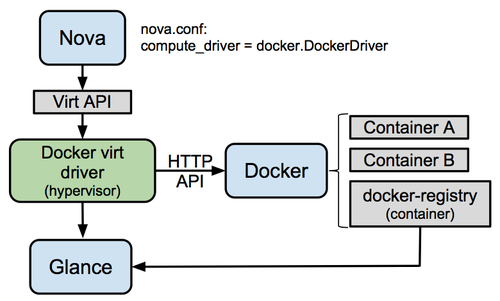
\includegraphics[scale=0.5]{dockeropenstackmodule}
  \caption[Docker module for Openstack working schema]{Docker module for
    Openstack working schema~\cite{openstackDockerModule}}
  \label{chap:archimpl:sec:fistattempt:img:dockeropnestackmodule}
\end{figure}

After the initial Openstack and Openbaton configuration we started making the
components talking to each other. First, we tried a simple \verb!iperf! data
transmission with two VNFs deployed by Openbaton as a common hypervisor-based
Openstack instances, as explained in~\cite{openbatonIperf}. With this test
completed, we started tinkering Openstack for using Docker containers instead of
traditional hypervisor instances. When we started developing this solution, we
adopted the Zun module, that aims to smoothly integrate Docker in Openstack.
Unfortunately, we were not able to make it properly work, in particular, it was
not possible to open desired ports on the Docker containers. This lead to the
impossibility to perform packet forwarding between VNFs. On top of that, we
found difficulties regarding the integration of Docker images in TOSCA
definitions and Openstack. These two issues are related: the TOSCA definition
does not have any keyword to specificate in any way that the image used for the
VNF definition is a Docker image, and Openstack, with the Zun plugin, at the
time of the implementation did not performed the image pull from any Docker
registry. The impossibility to easily set the containers ports and the lack of
some support between the TOSCA definition and the Openstack Zun plugin pushed us
to drop Openstack as a possible solution and to start looking for another valid
VIM component.

\section{Second attempt}

After the failure to find a viable setting for Openstack, we decided to look
around for other solutions. We started studying proper Docker container
orchestrators that could offer all the features we needed: container lifecycle
management, scaling, healing and monitoring. We decided to pick two of the most
mature and famous ones: Docker Swarm and Kubernetes. The decision to study only
these two relies on their big community supporting them and the possibility to
easily found projects that used the aforementioned frameworks.

\subsection{Docker Swarm}

\begin{figure}[t]
  \centering
  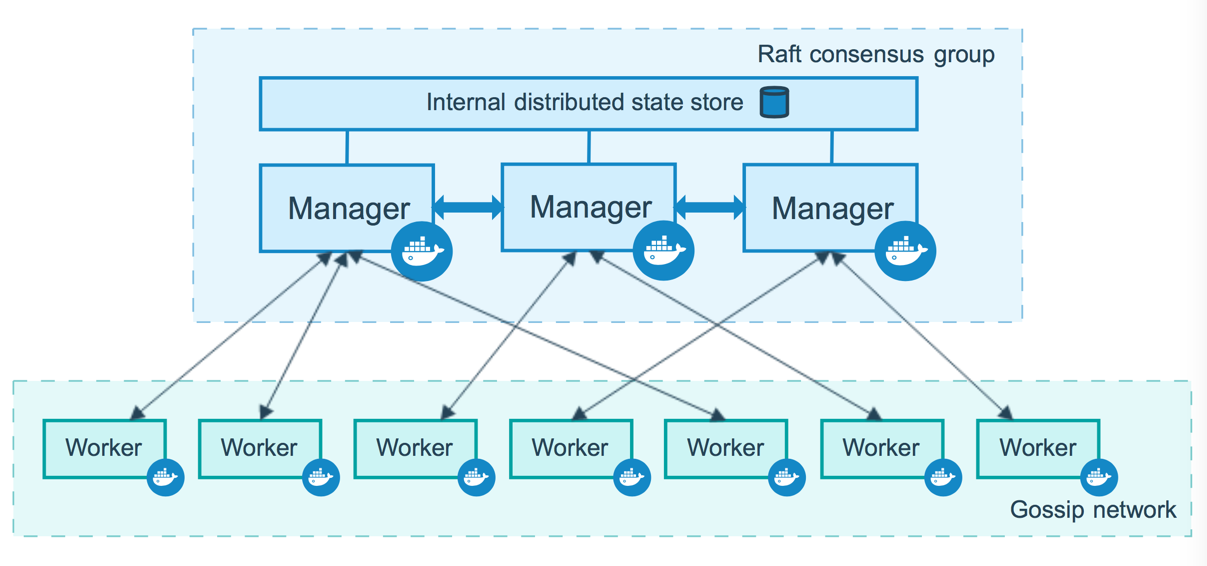
\includegraphics[scale=0.35]{swarm_diagram}
  \caption[Docker Swarm schema]{Docker Swarm schema~\cite{dockerSwarmWiki}.}
  \label{chap:archimpl:sec:secondattempt:img:dockerswarm}
\end{figure}

First we started playing with Docker Swarm. Docker Swarm is a product directly
made by the Docker Inc., so it seamlessly integrates with other Docker tools
such as Docker Compose. The installation and set-up is pretty straightforward,
and the configuration is almost automatically handled by Docker itself. The
minimum number of nodes in order to create a proper Docker Swarm cluster is of
three, where one must be a manager node (designed to orchestrate the other
nodes in the cluster), while the others can be simple workers. Multiple managers
can coexist in the same cluster, as long as only one effectively operates. The
others act like backup manager in case the one orchestrating goes down for some
reason. The networking is given out-of-the box, and the same holds for
distributed persistence. While this for most of the uses cases can be considered
a pro, in our specific situation the impossibility to tweak the network
configuration was a cons, since it was important for us to have the full control
over the network, especially regarding the SFC implementation, explained better
in Chapter~\ref{chap:vnf_ns_impl}.

\subsection{Kubernetes}
Kubernetes, as already described in the technology section, is an orchestrator
created by Google able to create a software abstraction from the underlying
virtualization technology. This enables Kubernetes to create an integration with
Docker. Kubernetes has an architecture based on plug-ins, giving the possibility
to the users to change part of Kubernetes itself, such as the networking routing
strategy or the persistence layer. With this flexibility Kubernetes offered to
us what Docker Swarm was not able to give. Additionally, we had the possibility
to set custom Domain Name System (DNS) lookups and distribute other internal
components in order to avoid requests bottleneck.

\subsection{Kubernetes configuration}
\label{chap:archimpl:sec:secondattempt:sec:k8s}
\begin{figure}[t]
  \centering
  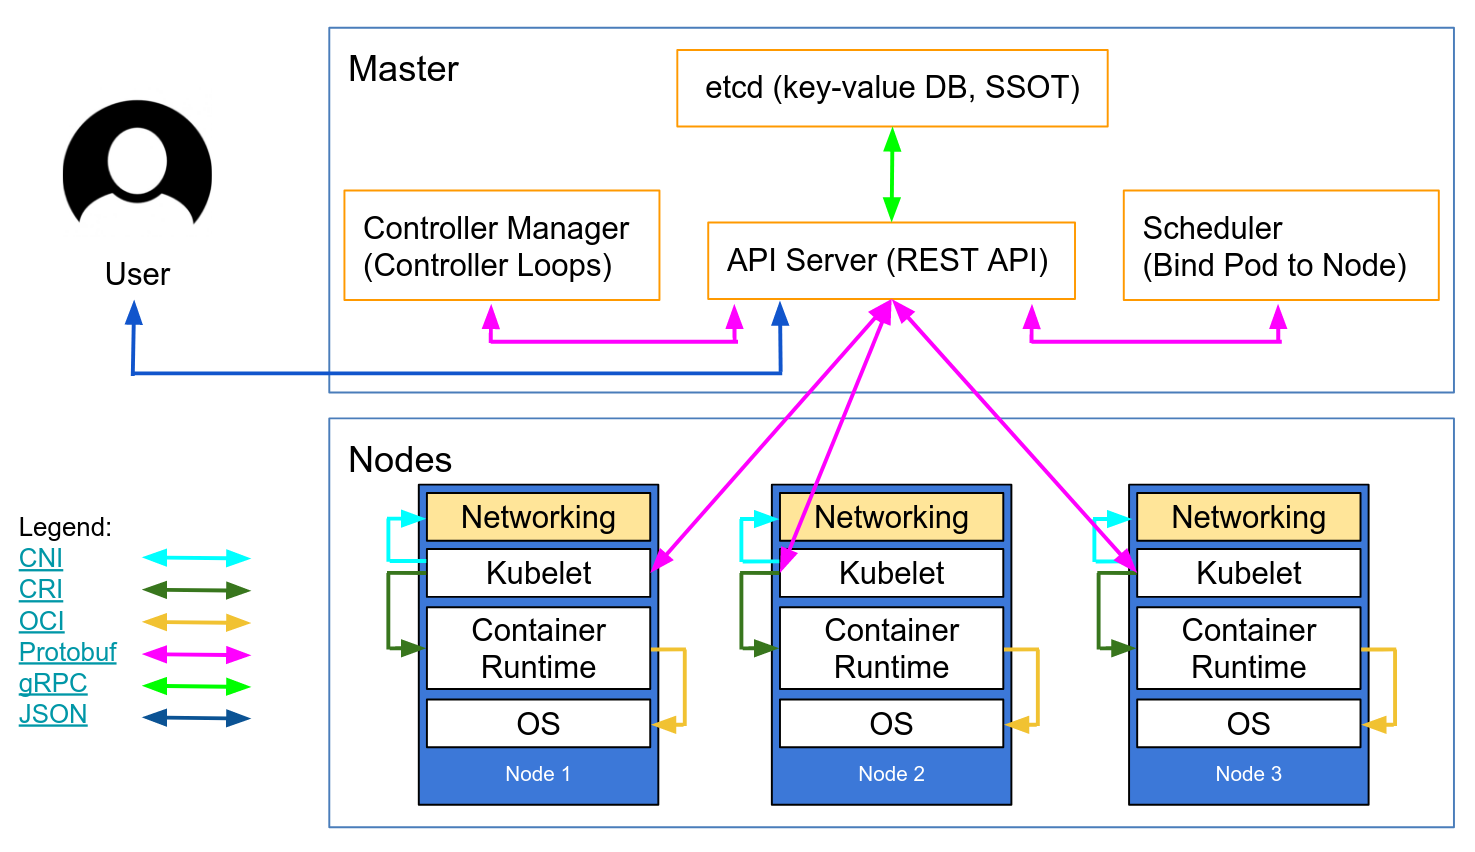
\includegraphics[scale=0.25]{kubernetes-control-plane}
  \caption[Kubernetes control plane schema]{Kubernetes control plane
    schema~\cite{k8scp}. It is possible to denote important components in the
    Kubernetes Control plane. In this high-level component architecture the
    master keeps an internal database, \emph{etcd}, the entry point for the API
    Server and the Pod scheduler. The nodes instead contain the kubelet daemon,
    the container runtime and the networking configuration.}
  \label{chap:archimpl:sec:secondattempt:img:k8scp}
\end{figure}

Kubernetes does not have a minimum number of nodes in order to properly work.
Nonetheless, we decided to use a four node cluster configured in the following
way: three slaves nodes (also known as \emph{minions}) and one master node. The
Kubernetes version installed was the 1.11, enabling us to exploit new features
like a reworked DNS lookup system and new storage features\footnote{A full
  kubernetes log release can be found at:
  \url{https://kubernetes.io/blog/2018/06/27/kubernetes-1.11-release-announcement/}}.
We initially deployed from the internal Openstack of the University four nodes
with 4GB of RAM, 10 GB of SSD storage and 2 vCPUs on Ubuntu 16.04 machines (that
we later swapped with CentOS 7). We performed the installation using the
official Kubernetes repositories. After the initial installation, we obtained a
configuration similar to the one illustrated in
Figure~\ref{chap:archimpl:sec:secondattempt:img:k8scp}. In this figure is
possible to denote different components on the master node and on the minions,
which will be described.

\subsubsection{Master architecture}
\begin{description}
\item[API Server] Fist of all, the User interacts with an API Server located in
  the master node. These APIs are developed using the Swagger tool, ensuring
  consistency and uniformity. From the image, is possible to see that the API
  Server communicates with all the main components of the architecture.
\item[etcd] The \verb!etcd! component communicates via the gRCP protocol, an
  efficient Remote Procedure Call (RPC) protocol to serve data to the API
  Server. This component is a distributed key-value storage, and allows data to
  be shared in a reliable way across different machines~\cite{etcddatamodel}.
\item[Controller Manager] The Controller Manager is the main Kubernetes control
  loop, and its role is to periodically check the system health and integrity.
  It communicates with the API Server via the Protobuf protocol, a
  language-neutral, platform-neutral and extensible data serialization
  mechanism.
\item[Scheduler] The Scheduler regulates the Pods distribution in the minions,
  having a knowledge of the current cluster typology and of the current
  resources available. On top of that, it is able to handle hardware
  constraints, defined policy, and defined class of QoS.
\end{description}

All of the previously descripted components are hidden behind the API server,
which is the only component the final user can really interact with. The
communication protocol between the API server and the final user used is a
common JSON data object interchange. To make the Kubernetes more human-friendly,
Kubernetes comes with a command line interface (CLI) tool, called
\verb!kubectl!, that allows to easily perform deployments and admin operations
on the cluster without having a full knowledge of the official API.

\subsubsection{Minions architecture}

As referred in Figure~\ref{chap:archimpl:sec:secondattempt:img:k8scp}, the API
server interacts with the components located in the minion nodes. In the image
we can denote different modules.
\begin{description}
\item[Kubelet] The \verb!kubelet! daemon is the core component that runs in
  every minion, and \emph{de facto} acts like a local manager. It receives YAML
  or JSON definitions from the API Server of Pod specifications (PodSpec) that
  have to be deployed in the node where is running. Then, its role is to ensure
  that the Pods deployed are up and healthy. This excludes possible
  interference with other virtualized deployments.
\item[Container Runtime] This runtime does not have to necessarily be based on
  Docker or a container-based technology, but it can be based on an hypervisor
  one, e.g. the KuberVirt project\footnote{Additional information about this
    project can be found at the following link: \url{https://kubevirt.io/}}. The
  container runtime performs the real Pods deployments.

  Communications between the container runtime and the Kubelet component are
  performed by the Container Runtime Interface (CRI), that consists of a series
  of specifications/requirements built on top of the Protobuf protocol API.
  Additionally, the Container Runtime has to communicate with the underlying OS,
  and this operation is performed using the Open Container Initiative (OCI)
  specification, which seeks to provide a standard on how to interact and run
  the container images on the host OS.
\item[Networking] This part aims to provide to the container runtime network
  connectivity. The role of the networking module is to provide, over than the
  standard Internet connectivity, the possibility for Pods to see each other as
  a part of the same network, even if Pods could be dislocated in other minions
  working between different subnets or completely different network domains. On
  top of that, dynamic port allocation has to be kept in consideration too. The
  Kubernetes networking model focus on three fundamental
  requirements~\cite{k8snetworkingwiki}:
  \begin{itemize}
  \item all containers have to communicate with all the other containers without
    NAT;
  \item all nodes have the possibility to communicate with all containers (and
    vice-versa) without NAT;
  \item the IP that a container sees itself as is the same IP that others see it
    as.
  \end{itemize}
  It is important to note that the IP addresses are at the Pod scope and not at
  the container one. Every Pod has in fact its own networking space. Containers
  inside a Pod can reach each other using the \verb!localhost! address. In
  Kubernetes, several networking implementations exist, like Flannel, Google
  Compute Engine (GCE), Kube-route, Project Calico~\cite{k8snetworkingwiki}. For
  our deployment, we decided to use Flannel, that demonstrated to work without
  any particular configuration and to be mature enough to handle big workloads.

  The communications between this component and the Kubelet one are carried
  through the Cloud Native Interface (CNI) protocol, that consists of a set
  of specification and libraries for writing plugins to configure network
  interfaces in Linux containers~\cite{cnigithub}.
\end{description}

\subsection{Openbaton integration}

\begin{figure}[t]
  \centering
  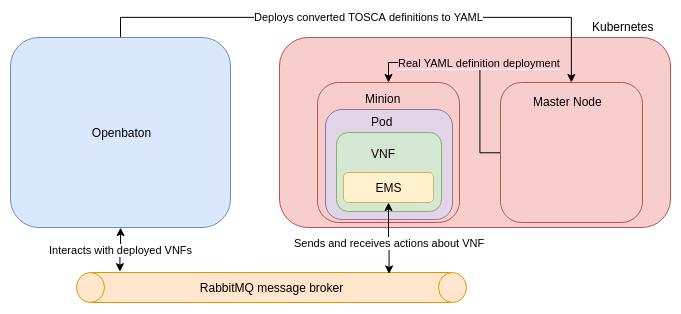
\includegraphics[scale=0.5]{Attempt2v1}
  \caption[Second attempt components organization schema]{Second attempt
    components organization schema. It is possible to see, differently from the
    first attempt, how now Kubernetes covers the old Openstack role and act as
    VIM, receiving YAML definitions in to the master node that will schedule the
    VNF in one of its minions.}
  \label{chap:archimpl:sec:secondattempt:img:schema1}
\end{figure}

After the Kubernetes configuration and installation, we started working for a
viable integration between Kubernetes and Openbaton. Our first idea is the one
illustrated in Figure~\ref{chap:archimpl:sec:secondattempt:img:schema1}:
Openbaton, that usually handles the TOSCA definitions storing them in its
database, had to somehow convert these definition in a suitable YAML for
Kubernetes, that had in turn to elaborate it and schedule to one minion in the
cluster. The monitoring and management would remain untouched, as we planned to
create an image with the integrated EMS tools that provided a seamless
integration with Docker container. With this setting, the only thing to solve
was how to convert TOSCA definitions in YAML one. The first thing we started
thinking about was how to perform the conversion. This topic was quite important
because the TOSCA definition does not really consider the possibility to have an
alternative virtualization system apart from the hypervisor one. This causes the
TOSCA definition to be, in our opinion, too much focused on the resources usage
and granularity aspects such the deployment flavour and the kind of virtual link
(concept that does not really exists in container based systems) to instantiate.
Nonetheless, we performed a mapping between most of the TOSCA keywords with some
of the YAML definitions, in a way that a TOSCA configuration file was able to
generate a valid YAML deployment. After that, we started thinking instead who,
in the current architecture, had the task to perform this operation. Initially
we thought that Kubernetes itself could have been a perfect candidate. From a
received TOSCA, a Kubernetes component should have validated and translated the
TOSCA definition to generate a YAML suitable to be finally submitted to the
Kubernetes API Server. Another feasible approach could have been to create a
Openbaton plugin in order to convert the TOSCA definition before submitting it
to Kubernetes for the deployment. This solution had great advantages in terms of
responsibility separation: in this way only the MANO had to know, for a VIM
based on Kubernetes, that a conversion was needed. From a Kubernetes
point-of-view, nothing would have changed, since all the configuration
conversion would have been performed by Openbaton.

\begin{figure}[t]
  \centering
  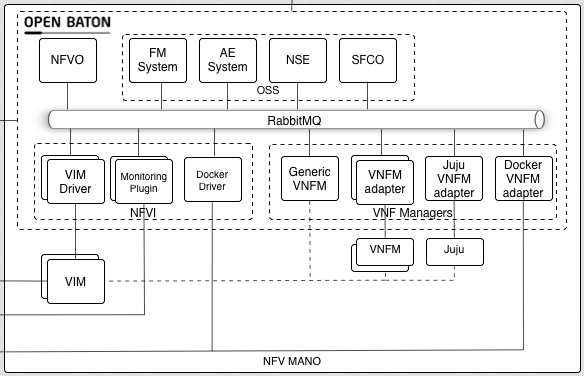
\includegraphics[scale=0.7]{OpenbatonMANO}
  \caption[Openbaton architecture components]{Openbaton architecture components,
    taken from~\cite{openbatondocumentation}.}
  \label{chap:archimpl:sec:secondattempt:img:openbatonMANO}
\end{figure}

We started inspecting the Openbaton framework, to identify possible modules
where the conversion should have taken place. We identified first the VIM
driver, that is the component that directly interacts with the VIM, and then the
VNFM, because we discovered there were programmatic dependencies between the two
Openbaton default components. After we identified the VIM driver and the VNFM as
components to be rewritten and to be adapted to the Kubernetes VIM, we studied
the original components code. We discovered that regarding these components the
documentation was very poor, especially looking the code. On top of that, the
program interfaces given by the developers did not match our expectations: we
thought to find interfaces independent from the type of the virtualization
technology, instead, we found that they were strictly coupled with frameworks
like Openstack or cloud vendors like Google Compute engine or Amazon AWS. These
reasons, with the fact that after two weeks we were not able to get any working
prototype of VIM driver or VNFM we gave up, searching for another solution.

\section{Final Design: End-to-end MANO}

The impossibility to develop a custom VIM driver and VNFM manager led us to
search for an alternative solution. Then, we started to work directly on the
VIM. The base approach was to create an API Server which in future an Openbaton
plugin could contact and simply deploy TOSCA definitions, interacting with a set
of RESTful APIs. We called this simple backend \emph{Harbor}.

\subsection{Harbor: extending the capabilities}
\label{chap:archimpl:sec:secondattempt:sub:harbor}
Harbor grew considerably during the project development, as it revealed to be a
key component of our architecture. Harbor does not have a web interface, but as
already written it has a RESTful API that allows users to interact with it using
CRUD operations. It offers functionalities similar to Openbaton: possibility to
save and retrieve VNFs and SFCs definitions. When an SFC is saved, a consistency
check is performed to assure that all the VNFs have already been defined in
Harbor. On an SFC deployment, with a mechanism similar to the Openbaton one, all
the associated VNFs are set up too, making the whole operation of launching a
SFC atomic from the user point-of-view. Since this architecture component grew
until it became a Kubernetes MANO, we added a feature that, in our opinion,
Openbaton lacks: smart resource utilization. Harbor, in fact, during an SFC
deletion, checks if any related VNF remains orphan (which means without any SFC
using it). In that case the VNF will enter in a state of pruning: after five
minutes, if the VNF has not be re-utilized by any other SFC it will be deleted.
This mechanism assure faster deployments in environments where NSs are
continuously taken up and down.

\begin{figure}[t]
 \centering
 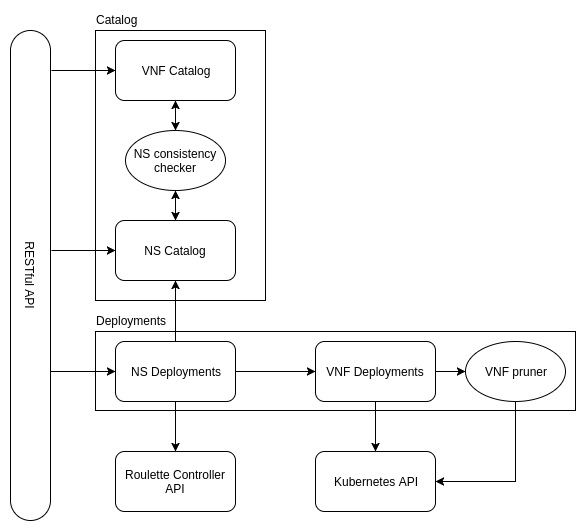
\includegraphics[scale=0.5]{Harbor_architecture}
 \caption[Harbor architectural schema]{Harbor architectural schema}
 \label{chap:archimpl:sec:secondattempt:img:harborarchitecture}
\end{figure}

\subsection{The need for additional components}

\begin{figure}[t]
  \centering
  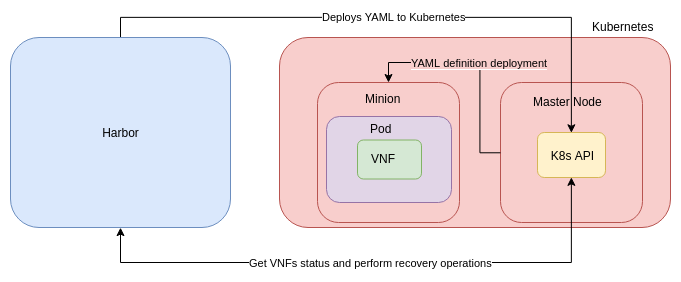
\includegraphics[scale=0.5]{Attempt2v1Harbor}
  \caption[Second attempt revision one schema]{Second attempt revision one
    schema. It is possible to see how Harbor completely substituted Openbaton.
    Additionally, Harbor now operates directly with the Kubernetes API,
    retrieving information about the VNFs status from it. This causes the VNFs
    to be lighter because they don't have to include any reporting tools, like
    the EMS, in it.}
  \label{chap:archimple:sec:secondattempt:img:attempt2v1harbor}
\end{figure}

Terminated the Harbor development, we ended up in a situation similar the one
depicted in Figure~\ref{chap:archimple:sec:secondattempt:img:attempt2v1harbor}.
It is possible to see how the Openbaton framework is not necessary anymore:
Harbor, in fact, ended up substituting it. We then started to think about the
challenges of integrating the SFC structure inside a Kubernetes cluster. We
identified the following challenges:
\begin{itemize}
\item whole system scalability: we wanted that every component had the
  possibility to scale during intense workloads, without the necessity of human
  intervention.
\item ingress and egress points: there should be at least two points in the
  cluster were the packet enters and exits;
\item dynamic package routing: as formulated by one of our requirements, packet
  routing had to be dynamic. We immediately identified a possibility to create
  this functionality with the already-built features of Kubernetes;
\item a framework to automatically forward the data elaborated by the VNF: we
  identified the possibility to build a framework that automatically handled the
  packet receiving from another VNF, it properly called the function that had to
  elaborate the packet payload and then it forwarded the result to the next VNF;
\item connection status: having ingress and egress points implicates the
  necessity to save some persistent data in a distributed manner.
\end{itemize}

\subsubsection{Scalability considerations}
When adopting Kubernetes, we realized the possibility to make every component
easily scalable. Indeed, all the following components can be described in
Kubernetes as a \verb!Service!. For a \verb!Service! a consequent
\verb!Deployment! can be associated, giving the possibility for it to scale
under heavy workloads. The introduction of scalability meant that it was not
possible to refer to the components based on their IP, but we had to refer to
their service name. As it will be explained later, this introduced challenges
especially for the ingress and egress points of our network, that have to keep a
connection with the sender and the receiver. On top of that, the scalability and
the required DNS lookups meant a possible bottleneck. With a great number of
components and VNFs constantly querying the centralized Kubernetes DNS lookup
system a performance degradation could have easily happened. We decided to
distribute the DNS service too, integrating the CoreDNS Kubernetes default
service with \emph{Dnsmasq}, a DNS server able to perform query caching for
faster name resolution. We created a Dnsmasq \verb!DaemonSets!, which in turn
deployed one Pod with Dnsmasq running inside for every minion in the cluster. At
the time of the VNF launch, we set that the DNS resolution should pass first for
the local Dnsmasq DNS, and then for the Kubernetes CoreDNS service. In this way,
we were able to distribute the DNS query workload from the master, using a local
caching system to speed up the name resolution between services.

\subsubsection{Ingress and Egress: Ironhide}
As just said, the whole framework needs to have and entry and an exit point.
These, defined as \emph{Ingress} and \emph{Egress} points, are performed by
\emph{Ironhide}. Ironhide hides the whole packet processing to the sender $S$
and the receiver $R$. When a client $S$ performs a request to $R$, the packet
actually goes through Ironhide, who has an internal classifier that it is able
to recognize the type of connection and to choose the right NS the packet has to
go through. This process is fundamental since it keeps the connection between
$S$ and $R$ up, for both TCP and UDP based communications. Since the connection
needs to be end-to-end, the state of the connections are saved in the
\emph{Roulette Controller} component.

\subsubsection{Dynamic package routing: the Roulette component}
\label{chap:prjan:sec:tech:sub:SFC:sub:roulette}
Dynamic end-to-end communications between VNFs would not be possible without a
third component acting as a route controller. Roulette fulfills this role,
providing a back-end where the single Service Function Forwarder (SFF) can ask
the next packet hop. Indeed, routes must be submitted by another component, that
we identified as Harbor. After a NS deployment, Roulette gets instructed with a
new route describing a NS. Every NS has a proper ID (called \verb!sfid!), and
thus when the classifier checks a packet typology, it labels that packet with
the specific NS ID (for a detailed description about the SFC header see
Section~\ref{chap:background:sec:sfc}). Finally, thanks to this label, every VNF
knows the packet's chain and it will correctly forward the it to the next VNF.

\subsubsection{Keeping the connection status}
The scalability challenge introduces new issues in the system. The most
important is keeping up stateful connections, since the ingress and egress
points could be more than one container. With this consideration in mind, we
started thinking at how and where keeping information about the ingress
container handling the connection with the sender $S$ and about the egress
container talking with the receiver $R$. Since the Roulette component has a
complete end-to-end topology view of the system, we decided to store these
additional information (we called it \emph{endpoints}) in it.

\subsubsection{A Service Function Forwarder: Astaire}
As is possible to denote, an SFC-unaware VNF can not elaborate a packet directly
coming from an SFC. The packet coming from an SFC contains additional
information and metadata that have to be removed first. In this context, we
decided to build a framework, Astaire, that could kept the SFC related details
decoupled from the core of the VNF, in other words, the entity that actually
elaborates the packet. Built using an event-based pattern, it presents hooks
that allow other software written in different languages from the Astaire one
(e.g. Java), to be called dynamically at runtime in order to process the packet.
The result of this elaboration gets returned to Astaire, that performs the
beforehand cited operations of VNFs communication and forwarding. In the SFC
specification, Astaire is defined as a SFF.

\subsection{Discussion}
At the end, we were able to create a scalable architecture that followed the
ETSI MANO standard, with Kubernetes as VIM and Harbor has MANO. We faced
additional challenges regarding the system scalability, that we solved using the
Roulette controller. We eased the creation of VNFs with Astaire, and we created
proper ingress and egress points with Ironhide, that supported scalability
issues and performed a protocol-based packet classification. Is possible to see
a final architectural schema in
Figure~\ref{chap:archimpl:sec:secondattempt:img:attempt2v1total}.

\begin{figure}[t]
  \centering
  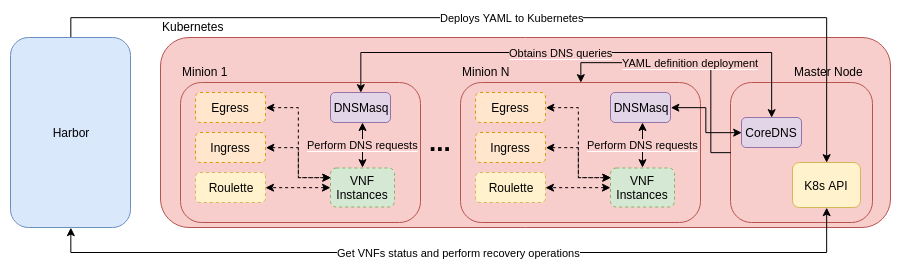
\includegraphics[scale=0.48]{Attempt2v1Total}
  \caption[Final components organization]{Final components organization. In the
    image is possible to denote how Egress, Ingress, the Roulette Controller and
    the VNFs instances are optional or could not be present in the minion, while
    DNSMasq is always deployed.}
  \label{chap:archimpl:sec:secondattempt:img:attempt2v1total}
\end{figure}
